%iffalse
\documentclass[journal]{IEEEtran}
\usepackage[a5paper, margin=10mm]{geometry}
%\usepackage{lmodern} % Ensure lmodern is loaded for pdflatex
\usepackage{tfrupee} % Include tfrupee package


\setlength{\headheight}{1cm} % Set the height of the header box
\setlength{\headsep}{0mm}     % Set the distance between the header box and the top of the text


%\usepackage[a5paper, top=10mm, bottom=10mm, left=10mm, right=10mm]{geometry}

%
\usepackage{gvv-book}
\usepackage{gvv}
\setlength{\intextsep}{10pt} % Space between text and floats

\makeindex

\begin{document}
\bibliographystyle{IEEEtran}
\onecolumn
%endif

\title{2021-February Session-02-26-2021-shift-1-16-30}
\author{AI24BTECH11031 - Shivram S}
\maketitle
\bigskip

\renewcommand{\thefigure}{\theenumi}
\renewcommand{\thetable}{\theenumi}

\begin{enumerate}
    \item If $\lambda_1$ and $\lambda_2$ are the wavelengths of the third member of
    Lyman and the first member of the Paschen series respectively, then the value
    of $\lambda_1:\lambda_2$ is

    \begin{multicols}{4}
    \begin{enumerate}
        \item $1:3$
        \item $1:9$
        \item $7:135$
        \item $7:108$
    \end{enumerate}
    \end{multicols}

    \item The temperature $\theta$ at the junction of two insulating sheets, having
    thermal resistances $R_1$ and $R_2$ as well as the bottom and top temperatures
    $\theta_1$ and $\theta_2$ (as shown in the figure) is given by:

    \begin{multicols}{2}
    \begin{enumerate}
        \item $\frac{\theta_1R_2 + \theta_2R_1}{R_1 + R_2}$
        \item $\frac{\theta_1R_2 - \theta_2R_1}{R_2 - R_1}$
        \item $\frac{\theta_2R_2 - \theta_2R_2}{R_2 + R_1}$
        \item $\frac{\theta_1R_1 + \theta_2R_2}{R_1 + R_2}$
    \end{enumerate}
    \end{multicols}

    \item In Young's double-slit experiment two slits are separated by $2 mm$ and the
    screen is placed one meter away. When light of wavelength $500 nm$ is used, the
    fringe separation will be:

    \begin{multicols}{4}
    \begin{enumerate}
        \item $0.75 mm$
        \item $0.50 mm$
        \item $1 mm$
        \item $0.25 mm$
    \end{enumerate}
    \end{multicols}

    \item Given below are two statements: one is labelled as Assertion A and the
    other is labelled as Reason R.

    \textbf{Assertion A}: An electron microscope can achieve better resolving power
    than an optical microscope.

    \textbf{Reason R}: The de Broglie's wavelength of the electrons emitted from an
    electron gun is much less than the wavelength of visible light.

    \begin{enumerate}
        \item A is true but R is false.
        \item Both A and R are true but R is NOT the correct explanation of A.
        \item Both A and R are true and R is the correct explanation of A.
        \item A is false but R is true.
    \end{enumerate} 

    \item Four identical solid spheres each of mass $m$ and radius $a$ are placed
    with their centres on the four corners of a square of side $b$. The moment of
    inertia of the system about one side of square where the axis of rotation is
    parallel to the plane of the square is:

    \begin{center}
    \begin{tikzpicture}
        \draw (0, 0) circle (0.5) node {a};
        \draw [<->] (0, 0.5) -- (0, 2.5) node[midway, above right] {b};
        \draw (0, 3) circle (0.5) node {a};
        \draw [<->] (0.5, 0) -- (2.5, 0) node[midway, above] {b};
        \draw (3, 3) circle (0.5) node {a};
        \draw [<->] (3, 2.5) -- (3, 0.5) node[midway, above left] {b};
        \draw (3, 0) circle (0.5) node {a};
    \end{tikzpicture}
    \end{center}
    
    \begin{multicols}{4}
    \begin{enumerate}
        \item $\frac{4}{5} ma^2$
        \item $\frac{8}{5} ma^2 + mb^2$
        \item $\frac{4}{5} ma^2 + 2mb^2$
        \item $\frac{8}{5} ma^2 + 2mb^2$
    \end{enumerate}
    \end{multicols}

    \item The normal density of a material is $\rho$ and its bulk modulus of
    elasticity is $K$. The magnitude of increase in density of material when a
    pressure $P$ is applied uniformly on all sides, will be:

    \begin{multicols}{4}
    \begin{enumerate}
        \item $\frac{\rho K}{P}$
        \item $\frac{K}{\rho P}$
        \item $\frac{P K}{\rho}$
        \item $\frac{\rho P}{K}$
    \end{enumerate}
    \end{multicols}

    \item LED is constructed from Ga-As-P semiconducting material. The energy gap of
    this LED is $1.9 eV$. Calculate the wavelength of light emitted and its colour.

    \begin{multicols}{2}
    \begin{enumerate}
        \item $654 nm$ and red colour
        \item $1046 nm$ and blue colour
        \item $1046 nm$ and red colour
        \item $654 nm$ and orange colour
    \end{enumerate}
    \end{multicols}

    \item Five equal resistances are connected in a network as shown in the figure.
    The net resistance between points A and B is:

    \begin{center}
    \begin{circuitikz}
        \draw (0, 0) node[left]{E}
            to[R=R]
            (3, 5.18) node[above]{D}
            to[R=R]
            (6,0) node[right]{C}
            to[R=R]
            (0,0);
        \draw (0, 0)
            to[R=R]
            (3, 1.73)
            to[R=R]
            (3, 5.18);
        \draw (3, 1.73) -- (4, 1.15) node[above]{A};
        \draw (6, 0) -- (5, 0.578) node[above]{B};
    \end{circuitikz}
    \end{center}

    \begin{multicols}{4}
    \begin{enumerate}
        \item $\frac{3R}{2}$
        \item $\frac{R}{2}$
        \item $R$
        \item $2R$
    \end{enumerate}
    \end{multicols}

    \item Find the gravitational force of attraction between the ring and sphere as
    shown in the diagram, where the plane of the ring is perpendicular to the line
    joining the centres. If $\sqrt{8}R$ is the distance between the centres of a
    ring (of mass $m$) and a sphere (of mass $M$) where both have equal radius $R$.

    \begin{center}
    \begin{tikzpicture}
        \draw (0, 2) ellipse (0.5 and 1.5) node[left] {X};
        \draw (0, 2) -- (0, 3.5) node[midway, above right] {R};
        \draw (0, 3.5) node[above] {m};
        \draw (0, 2) -- (4, 2) node[midway, below] {$\sqrt{8}R$};
        \draw (4, 2) circle (1.5) node[right] {Y};
        \draw [->] (4, 2) -- (4, 0.5) node[midway, right] {R};
        \draw (4, 3.5) node[above] {M};
        \draw (0, 3.5) -- (4, 2);
        \draw (3, 1.95) node[above] {$\theta$};
    \end{tikzpicture}
    \end{center}

    \begin{multicols}{4}
    \begin{enumerate}
        \item $\frac{\sqrt{8}}{9} \frac{GmM}{R^2}$
        \item $\frac{\sqrt{8}}{27} \frac{GmM}{R^2}$
        \item $\frac{2\sqrt{2}}{3} \frac{GmM}{R^2}$
        \item $\frac{1}{3\sqrt{8}} \frac{GmM}{R^2}$
    \end{enumerate}
    \end{multicols}

    \item Assume that a tunnel is dug along a chord of the earth, at a perpendicular
    distance $\frac{R}{2}$ from the earth's centre, where $R$ is the radius of the
    Earth. The wall of the tunnel is frictionless. If a particle is released in this\
    tunnel, it will execute a simple harmonic motion with a time period:
 
    \begin{multicols}{4}
    \begin{enumerate}
        \item $2\pi \sqrt{\frac{R}{g}}$
        \item $\frac{1}{2\pi} \sqrt{\frac{R}{g}}$
        \item $\frac{2\pi R}{g}$
        \item $\frac{g}{2\pi R}$
    \end{enumerate}
    \end{multicols}

    \item Find the electric field $E$ at point $P$ (as shown in the figure) on the
    perpendicular bisector of a uniformly charged thin wire of length $L$ carrying a
    charge $Q$. The distance of the point $P$ from the centre of the rod is
    $a = \frac{\sqrt{3}}{2}L$. 
     
    \begin{center}
    \begin{tikzpicture}
        \draw (0.2, 0) node[right] {Q} rectangle (0, 3);
        \draw [<->] (-0.2, 0) -- (-0.2, 3) node[midway, left] {L};
        \draw [dashed] (0.2, 1.5) node[below right] {O} -- (2.2, 1.5) node[below] {P};
        \draw [<->] (0.2, 2) -- (2.2, 2) node[midway, above] {a} node[above] {E};
    \end{tikzpicture}
    \end{center}

    \begin{multicols}{4}
    \begin{enumerate}
        \item $\frac{Q}{2\sqrt{3}\pi\varepsilon_0 L^2}$
        \item $\frac{\sqrt{3}Q}{4\pi\varepsilon_0 L^2}$
        \item $\frac{Q}{3\pi\varepsilon_0 L^2}$
        \item $\frac{Q}{4\pi\varepsilon_0 L^2}$
    \end{enumerate}
    \end{multicols}

    \item Given below are two statements: one is labelled as Assertion A and the
    other is labelled as Reason R.

    \textbf{Assertion A}: Body P having mass $M$ moving with speed $u$ has head-on
    collision elastically with another body Q having mass $m$ initially at rest.
    If $m << M$, body Q will have a maximum speed equal to $2u$ after collision.
    
    \textbf{Reason R}: During elastic collision, the momentum and kinetic energy are
    both conserved.
    
    In the light of the above statements, choose the most appropriate answer from the
    options given below:

    \begin{enumerate}
        \item A is correct but R is not correct.
        \item Both A and R are correct but R is NOT the correct explanation of A.
        \item A is not correct but R is correct.
        \item Both A and R are correct and R is the correct explanation of A.
    \end{enumerate}

    \item A short straight object of height $100 cm$ lies before the central axis of
    a spherical mirror whose focal length has absolute value $\abs{f} = 40 cm$. The\
    image of the object produced by the mirror is of height $25 cm$ and has the same
    orientation as the object. One may conclude from the information:

    \begin{enumerate}
        \item Image is real, same side of concave mirror.
        \item Image is virtual, opposite side of convex mirror.
        \item Image is virtual, opposite side of concave mirror.
        \item Image is real, same side of convex mirror.
    \end{enumerate}

    \item A particle is moving with uniform speed along the circumference of a circle
    of radius $R$ under the action of a central fictitious force $F$ which is
    inversely proportional to $R^3$. Its time period of revolution will be given by:

    \begin{multicols}{4}
    \begin{enumerate}
        \item $T \propto R^{5/2}$
        \item $T \propto R^2$
        \item $T \propto R^{4/3}$
        \item $T \propto R^{3/2}$
    \end{enumerate}
    \end{multicols} 

\end{enumerate}

\end{document}
